\documentclass[tikz,border=2pt]{standalone}
\usepackage[T1]{fontenc}
\usepackage[scaled=0.92]{helvet}
\renewcommand{\familydefault}{\sfdefault}
\usepackage{amsmath,amssymb}
\renewcommand{\tiny}{\fontsize{6.5}{7.5}\selectfont}
\renewcommand{\scriptsize}{\fontsize{7.5}{8.5}\selectfont}
\usetikzlibrary{arrows.meta,fit,backgrounds,calc,positioning}
\definecolor{cInk}{HTML}{22303C}
\definecolor{cGrp}{HTML}{0072B2}
\definecolor{cWarm}{HTML}{E69F00}
\tikzset{
  every node/.style={font=\scriptsize, text=cInk},
  done/.style={draw=cInk!75, rounded corners=2pt, fill=white, align=center, inner sep=3pt, minimum height=0.7cm},
  pend/.style={draw=cWarm!90!black, rounded corners=2pt, fill=cWarm!10, dash pattern=on 2.5pt off 1.8pt, thick, align=center, inner sep=3pt, minimum height=0.7cm},
  sysb/.style={draw=cGrp!80, rounded corners=2pt, fill=cGrp!7, align=left, inner sep=2pt, minimum height=0.42cm, text width=4.2cm, font=\tiny},
  arr/.style={-{Stealth[length=4pt,width=3pt]}, thick, draw=cInk!75},
  parr/.style={-{Stealth[length=4pt,width=3pt]}, thick, draw=cWarm!90!black, dash pattern=on 2.5pt off 1.8pt},
  panel/.style={draw=cInk!35, rounded corners=3pt, fill=cInk!3, inner sep=5pt},
  ptitle/.style={font=\scriptsize\bfseries, text=cInk!85, anchor=south west, inner sep=1pt},
}
\begin{document}
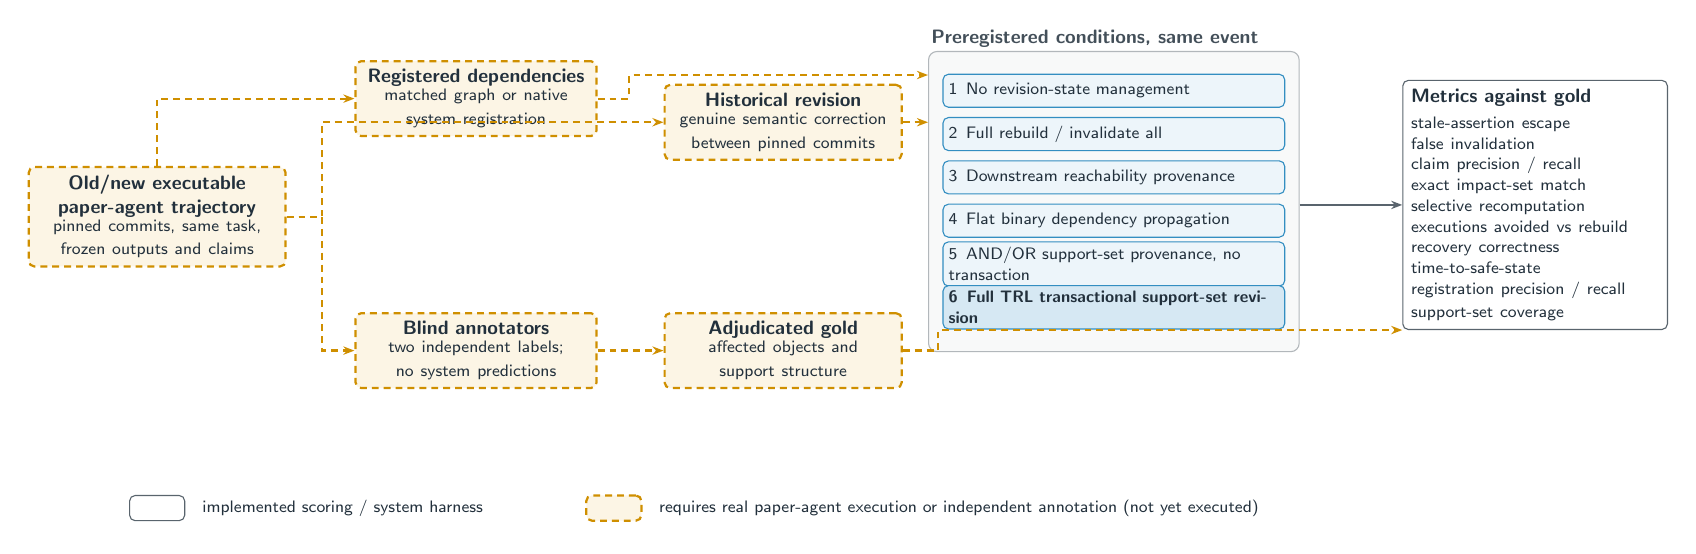
\begin{tikzpicture}[x=1cm,y=1cm]
% external trajectory and truth construction
\node[pend, text width=3.05cm] (traj) at (0,2.85) {\textbf{Old/new executable paper-agent trajectory}\\[-1pt]{\tiny pinned commits, same task,\\frozen outputs and claims}};
\node[pend, text width=2.85cm] (reg) at (4.05,4.35) {\textbf{Registered dependencies}\\[-1pt]{\tiny matched graph or native\\system registration}};
\node[pend, text width=2.85cm] (ann) at (4.05,1.15) {\textbf{Blind annotators}\\[-1pt]{\tiny two independent labels;\\no system predictions}};
\node[pend, text width=2.8cm] (gold) at (7.95,1.15) {\textbf{Adjudicated gold}\\[-1pt]{\tiny affected objects and\\support structure}};
\node[pend, text width=2.8cm] (mut) at (7.95,4.05) {\textbf{Historical revision}\\[-1pt]{\tiny genuine semantic correction\\between pinned commits}};
% implemented system conditions
\begin{scope}[shift={(12.15,0)}]
\node[sysb] (s1) at (0,4.45) {1\enspace No revision-state management};
\node[sysb] (s2) at (0,3.90) {2\enspace Full rebuild / invalidate all};
\node[sysb] (s3) at (0,3.35) {3\enspace Downstream reachability provenance};
\node[sysb] (s4) at (0,2.80) {4\enspace Flat binary dependency propagation};
\node[sysb] (s5) at (0,2.25) {5\enspace AND/OR support-set provenance, no transaction};
\node[sysb, fill=cGrp!16] (s6) at (0,1.70) {\textbf{6\enspace Full TRL transactional support-set revision}};
\begin{scope}[on background layer]
\node[panel, fit=(s1)(s6), inner ysep=8pt] (PS) {};
\end{scope}
\node[ptitle] at (PS.north west) {Preregistered conditions, same event};
\end{scope}
\node[done, text width=3.15cm, align=left] (met) at (17.5,3.0) {\textbf{Metrics against gold}\\[2pt]{\tiny stale-assertion escape\\false invalidation\\claim precision / recall\\exact impact-set match\\selective recomputation\\executions avoided vs rebuild\\recovery correctness\\time-to-safe-state\\registration precision / recall\\support-set coverage}};
% arrows
\draw[parr] (traj.east) -- ++(0.45,0) |- (ann.west);
\draw[parr] (traj.north) |- (reg.west);
\draw[parr] (traj.east) -- ++(0.45,0) |- (mut.west);
\draw[parr] (ann) -- (gold);
\draw[parr] (mut.east) -- (PS.west |- 0,4.05);
\draw[parr] (reg.east) -- ++(0.4,0) |- (PS.west |- 0,4.65);
\draw[arr] (PS.east |- 0,3.0) -- (met.west);
\draw[parr] (gold.east) -- ++(0.45,0) |- (met.south west);
% status legend
\begin{scope}[shift={(0,-0.85)}]
\node[done, minimum height=0.32cm, minimum width=0.7cm] at (0,0) {}; \node[anchor=west,font=\tiny] at (0.45,0) {implemented scoring / system harness};
\node[pend, minimum height=0.32cm, minimum width=0.7cm] at (5.8,0) {}; \node[anchor=west,font=\tiny] at (6.25,0) {requires real paper-agent execution or independent annotation (not yet executed)};
\end{scope}
\end{tikzpicture}
\end{document}
